\section{System Results}
\label{sec:results}
\subsection{Real multi-process runs}
\label{sec:real}
Table~\ref{tab:real} reports the six real runs on the clients' test slices, 283,090 to 295,566 rows per run, with no attackers. Known attacks are detected almost completely. The cascade's micro-recall is 0.9956 to 0.9989 and its macro-recall over the 13 attack classes present is 0.9939 to 0.9981. The booster alone reaches 0.9954 to 0.9981 micro-recall, so on known attacks the autoencoder adds between 0.0002 and 0.0008. The bootstrap booster, scored on the held-back part of the calibration set, reaches 0.9947 to 0.9980 accuracy and 0.9609 to 0.9871 macro F1 (Table~\ref{tab:filterhonest}).

\begin{table*}[t]
\centering
\caption{Six real multi-process runs (20 rounds, no attackers), scored on the clients' test slices. Recall columns: cascade macro- and micro-recall, booster-alone micro-recall, autoencoder-alone macro-recall. False-alarm columns: all benign test packets, the median client's packets, benign connections with half or more of their packets flagged, and the share of false-alarm packets that come from the ten largest benign connections.}
\label{tab:real}
\small
\begin{adjustbox}{max width=\linewidth}
\begin{tabular}{rrcccccccc}
\toprule
 & & \multicolumn{4}{c}{Recall on known attacks} & \multicolumn{4}{c}{False alarms} \\
\cmidrule(lr){3-6}\cmidrule(lr){7-10}
Clients & Seed & Macro & Micro & Booster & AE alone & Packets & Median client & Connections & Top-10 share \\
\midrule
10 & 42 & 0.9958 & 0.9974 & 0.9970 & 0.461 & 0.1275 & 0.0286 & 0.0034 & 0.94 \\
10 & 43 & 0.9947 & 0.9978 & 0.9971 & 0.463 & 0.0884 & 0.0313 & 0.0074 & 0.80 \\
10 & 44 & 0.9939 & 0.9956 & 0.9954 & 0.220 & 0.0248 & 0.0293 & 0.0039 & 0.89 \\
20 & 42 & 0.9981 & 0.9989 & 0.9981 & 0.718 & 0.0588 & 0.0322 & 0.0104 & 0.52 \\
20 & 43 & 0.9970 & 0.9980 & 0.9974 & 0.619 & 0.1628 & 0.0307 & 0.0076 & 0.87 \\
20 & 44 & 0.9972 & 0.9978 & 0.9972 & 0.709 & 0.1089 & 0.0296 & 0.0081 & 0.90 \\
\bottomrule
\end{tabular}
\end{adjustbox}
\end{table*}

\textit{False alarms.} The packet false-alarm rate varies from 2.5\% to 16.3\% across the six runs, and nearly all of it comes from the second stage: the booster alone flags 0.012\% to 0.046\% of benign packets. The packet rate is a poor summary, because a few very long benign connections dominate it. In the 10-client, seed-42 run, client 9 holds a benign connection of 11,764 packets that the autoencoder flags in full. In five of the six runs, 80 to 94\% of all false-alarm packets come from the ten largest benign connections, and 52\% in the sixth. The median client's packet rate is 2.9 to 3.2\% in every run, close to the 3\% the 97th-percentile threshold implies. Counted per connection, 0.34 to 1.04\% of the 10,765 to 12,519 benign test connections have half or more of their packets flagged (Fig.~\ref{fig:fa}). An operator who acts on connections would see roughly one false alarm per hundred benign connections. One who acts on packets would see many more, concentrated in a handful of long-lived sessions.

\begin{figure}[t]
\centering
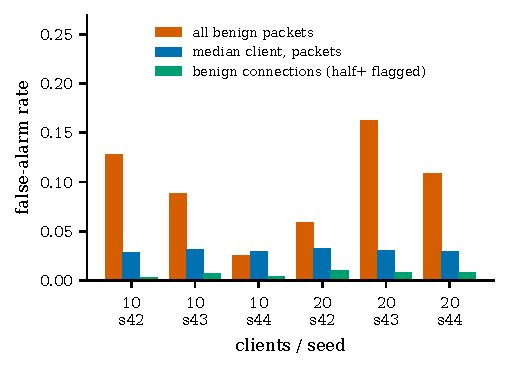
\includegraphics[width=\columnwidth]{figs/fig_fa.pdf}
\caption{False-alarm rate of the six real runs, counted three ways.}
\label{fig:fa}
\end{figure}

\textit{The autoencoder on its own.} Alone, the autoencoder detects between 22\% and 72\% of attack packets. It is weaker with 10 clients (0.220 to 0.463) than with 20 (0.619 to 0.718), and it varies strongly with the seed. Table~\ref{tab:perclass} shows why it still matters little for known attacks. Per class, the booster detects 0.984 to 1.000 and the cascade 0.987 to 1.000, while the autoencoder alone ranges from 0.037 on Backdoor to 0.939 on DDoS\_TCP. Its value lies in attack types the booster has never seen (Section~\ref{sec:zeroday}).

\textit{The filter with no attackers.} Even with no attacker present, the filter excluded 6 to 12 of 200 client-rounds in the 10-client runs and 12 to 19 of 400 in the 20-client runs (Table~\ref{tab:filterhonest}). Every exclusion but one was a MAD outlier. These are honest clients whose non-IID updates differ from the median, which is the confound discussed in Section~\ref{sec:discussion}.

\begin{table}[t]
\centering
\caption{Bootstrap booster scored on the held-back calibration rows, and honest client-rounds the trust filter excluded during each real run (no attackers present).}
\label{tab:filterhonest}
\small
\begin{adjustbox}{max width=\linewidth}
\begin{tabular}{rrccc}
\toprule
Clients & Seed & Accuracy & Macro F1 & Client-rounds excluded \\
\midrule
10 & 42 & 0.9947 & 0.9808 & 12 / 200 \\
10 & 43 & 0.9971 & 0.9609 & 6 / 200 \\
10 & 44 & 0.9980 & 0.9871 & 7 / 200 \\
20 & 42 & 0.9947 & 0.9808 & 19 / 400 \\
20 & 43 & 0.9971 & 0.9609 & 12 / 400 \\
20 & 44 & 0.9980 & 0.9871 & 12 / 400 \\
\bottomrule
\end{tabular}
\end{adjustbox}
\end{table}

\begin{table}[t]
\centering
\caption{Recall per attack type by stage, 10 clients, seed 42, with the range of cascade recall over all six real runs. MITM has no test rows (Section~\ref{sec:splits}).}
\label{tab:perclass}
\small
\setlength{\tabcolsep}{3pt}
\begin{adjustbox}{max width=\linewidth}
\begin{tabular}{lrcccc}
\toprule
Class & Test rows & Booster & AE alone & Cascade & Cascade, six runs \\
\midrule
Backdoor & 2,263 & 0.9885 & 0.037 & 0.9929 & 0.9729--0.9983 \\
DDoS\_HTTP & 6,915 & 0.9899 & 0.481 & 0.9899 & 0.9856--0.9963 \\
DDoS\_ICMP & 9,520 & 1.0000 & 0.317 & 1.0000 & 0.9997--1.0000 \\
DDoS\_TCP & 6,717 & 1.0000 & 0.939 & 1.0000 & 1.0000--1.0000 \\
DDoS\_UDP & 17,755 & 0.9999 & 0.306 & 1.0000 & 1.0000--1.0000 \\
Fingerprinting & 129 & 0.9845 & 0.070 & 0.9922 & 0.9730--1.0000 \\
Password & 7,795 & 0.9913 & 0.252 & 0.9914 & 0.9875--0.9963 \\
Port\_Scanning & 2,929 & 1.0000 & 0.684 & 1.0000 & 0.9982--1.0000 \\
Ransomware & 691 & 0.9841 & 0.488 & 0.9870 & 0.9847--0.9975 \\
SQL\_injection & 7,228 & 0.9990 & 0.894 & 0.9996 & 0.9976--1.0000 \\
Uploading & 5,567 & 0.9998 & 0.549 & 0.9998 & 0.9995--1.0000 \\
Vuln.\ scanner & 7,216 & 0.9946 & 0.501 & 0.9961 & 0.9925--0.9996 \\
XSS & 2,274 & 0.9960 & 0.471 & 0.9969 & 0.9893--0.9991 \\
\bottomrule
\end{tabular}
\end{adjustbox}
\end{table}

Phase~A took 1,063 to 1,844~s for 20 rounds (Table~\ref{tab:sizes}); 871 to 1,633~s of that is federated training, 16~s the calibration split, bootstrap classifier and client partition, and 156 to 191~s evaluation. Some runs shared the machine with other jobs, so these times are upper bounds.

\subsection{Ablation and poisoning sweep}
The in-process experiments reproduce the real runs closely. With no attackers, in-process attack macro-recall is 0.996, 0.996 and 0.994 for the three seeds, against 0.9958, 0.9947 and 0.9939 in the 10-client real runs. Table~\ref{tab:ablation} compares the five variants with three sign-flipping clients out of ten, and Table~\ref{tab:sweep} with Fig.~\ref{fig:poison} follows the full pipeline from 0\% to 50\% attackers.

\begin{table*}[t]
\centering
\caption{Ablation with 30\% sign-flipping clients, 10 clients, 20 rounds. Each cell lists seeds 42 / 43 / 44. The full-pipeline row is the sweep's 30\% point.}
\label{tab:ablation}
\small
\begin{adjustbox}{max width=\linewidth}
\begin{tabular}{llll}
\toprule
Variant & Attack macro-recall & AE-alone macro-recall & Benign FPR (packets) \\
\midrule
full\_pipeline & 0.995 / 0.997 / 0.995 & 0.490 / 0.373 / 0.245 & 0.1112 / 0.0653 / 0.0075 \\
plain\_fedavg & 0.992 / 0.994 / 0.990 & 0.013 / 0.002 / 0.092 & 0.0947 / 0.0301 / 0.0301 \\
trimmed\_mean\_only & 0.995 / 0.995 / 0.993 & 0.205 / 0.000 / 0.025 & 0.1070 / 0.0261 / 0.0299 \\
autoencoder\_only & 0.105 / 0.073 / 0.051 & 0.105 / 0.073 / 0.051 & 0.0473 / 0.0411 / 0.0445 \\
boosting\_only & 0.990 / 0.989 / 0.982 & -- & 0.0001 / 0.0001 / 0.0003 \\
\bottomrule
\end{tabular}
\end{adjustbox}
\end{table*}

\begin{table}[t]
\centering
\caption{Poisoning sweep, full pipeline, 10 clients, 20 rounds. Seeds 42 / 43 / 44.}
\label{tab:sweep}
\small
\setlength{\tabcolsep}{3pt}
\begin{adjustbox}{max width=\linewidth}
\begin{tabular}{rllll}
\toprule
Attackers & Attack macro-recall & AE-alone recall & Survival & Benign FPR \\
\midrule
0\% & 0.996 / 0.996 / 0.994 & 0.457 / 0.492 / 0.221 & -- & 0.118 / 0.041 / 0.035 \\
20\% & 0.995 / 0.996 / 0.994 & 0.466 / 0.483 / 0.258 & 0.30 / 0.40 / 0.23 & 0.105 / 0.094 / 0.037 \\
30\% & 0.995 / 0.997 / 0.995 & 0.490 / 0.373 / 0.245 & 0.50 / 0.55 / 0.62 & 0.111 / 0.065 / 0.008 \\
40\% & 0.994 / 0.994 / 0.992 & 0.297 / 0.139 / 0.074 & 0.60 / 0.64 / 0.61 & 0.091 / 0.038 / 0.043 \\
50\% & 0.995 / 0.990 / 0.985 & 0.249 / 0.000 / 0.000 & 0.64 / 1.00 / 0.99 & 0.115 / 0.052 / 0.030 \\
\bottomrule
\end{tabular}
\end{adjustbox}
\end{table}

\begin{figure*}[t]
\centering
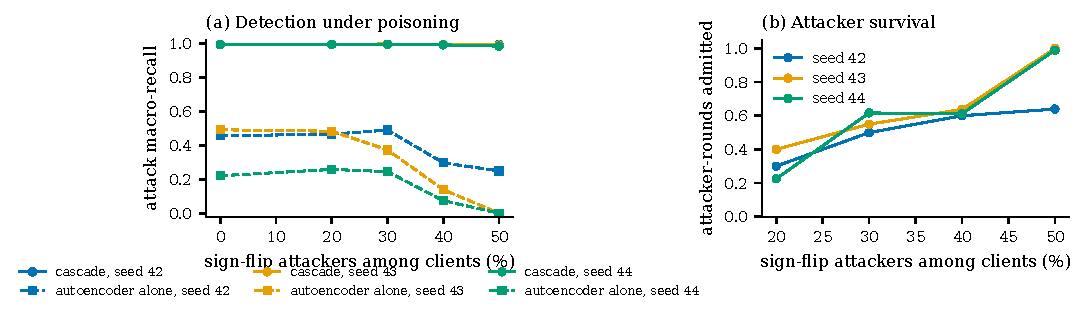
\includegraphics[width=\textwidth]{figs/fig_poison.pdf}
\caption{Full pipeline under increasing shares of sign-flipping clients, three seeds. (a) Known-attack macro-recall of the cascade (solid) and macro-recall of the autoencoder alone (dashed). (b) Share of attacker-rounds in which an attacker passed the filter.}
\label{fig:poison}
\end{figure*}

\textit{Known attacks are safe from poisoning.} Every variant that includes the booster keeps attack macro-recall between 0.982 and 0.997, and the full pipeline stays between 0.985 and 0.997 at every attacker fraction up to 50\%. The booster is trained on the server, so poisoned updates cannot reach it. Reported on its own, this number would hide what happens to the federated part.

\textit{Robust aggregation protects the autoencoder at 30\%.} The full pipeline's autoencoder detects 0.490, 0.373 and 0.245 at 30\% attackers, against 0.457, 0.492 and 0.221 with no attackers. Under plain FedAvg it detects 0.013, 0.002 and 0.092, and under the trimmed mean without the filter 0.205, 0.000 and 0.025. The trimmed mean alone fails because, with ten clients and a 15\% trim, it removes one update from each side, and three colluding attackers outnumber that. This is the expected breakdown of the rule~\cite{yin2018}. The margin over plain FedAvg is smallest at seed 44, where the autoencoder was weak to begin with.

\textit{The filter admits many attackers at this scale.} Attackers reached aggregation in 23 to 40\% of their rounds at 20\% attackers and in 50 to 62\% at 30\%. The autoencoder still holds at 30\%. Our reading, which we have not tested separately, is that the filter removes enough attackers for the stages after it to cope: at a survival of 0.50 to 0.62, about 1.5 to 1.9 of the three attackers pass in an average round, and the norm clip and one-per-side trim bound what they can do. At 40\% the autoencoder degrades to 0.297, 0.139 and 0.074. At 50\%, attackers are admitted in 64\%, 100\% and 99\% of their rounds and the autoencoder fails in two of three seeds. Once half the clients attack, the coordinate-wise median moves toward their direction, and any defence that takes the median as its consensus fails there.

\textit{The pre-filter matters.} Trained on all local traffic instead of boosting-filtered traffic, the autoencoder detects only 0.105, 0.073 and 0.051. Filtering out traffic the booster already recognises as attack leaves the autoencoder a much cleaner picture of benign behaviour.

\textit{The cascade's gain on known attacks is small and its false alarms vary.} Compared with boosting alone at 30\% attackers, the full pipeline gains 0.005 to 0.014 in macro-recall. Its packet false-alarm rate ranges from 0.75\% to 11.1\% across seeds, against at most 0.03\% for the booster alone. The spread follows the long-connection effect described above.

\subsection{Unseen attack types}
\label{sec:zeroday}
Fig.~\ref{fig:zeroday} and Table~\ref{tab:zeroday} report the leave-one-class-out experiment with no attackers. In all 42 cases (14 classes, three seeds), the cascade detects at least as much of the held-out class as the better of its two stages alone. Its mean detection rate over the 14 classes is 0.910, 0.944 and 0.895 for the three seeds, against 0.735, 0.757 and 0.723 for the classifier alone and 0.681, 0.728 and 0.590 for the autoencoder alone. The cost is a mean benign packet false-alarm rate of 0.079 to 0.104 across the held-out runs.

The held-out classes fall into three groups.

\textit{The classifier finds them anyway, under the wrong name.} DDoS\_ICMP, Fingerprinting, Port\_Scanning and Ransomware are detected at 0.982 or more by the classifier alone, because it maps each to a behaviourally similar class it knows. Held-out Port\_Scanning is labelled Fingerprinting in 99 to 100\% of rows, and held-out Ransomware is labelled Backdoor in 97 to 99\%. The detection counts, but an operator would see a confident alert with the wrong attack type.

\textit{Mostly the autoencoder finds them.} For DDoS\_UDP and MITM, the classifier alone detects 0.021 to 0.416 and 0.005 to 0.200. The cascade detects 0.803 to 0.905 and 0.751 to 1.000, almost all from the second stage. MITM is a single connection of 406 rows, so its numbers swing widely between seeds.

\textit{Hard for both, or seed-dependent.} Uploading is the weakest class in every seed (cascade 0.527 to 0.665). The classifier lets 70 to 80\% of it through as benign or with low confidence, and the autoencoder finds it only partly unusual. Backdoor (0.743 at seed 42, 0.998 otherwise) and Vulnerability\_scanner (0.859 at seed 44, 0.992 otherwise) depend on the seed, in both cases through the classifier alone, which detects 0.486 and 0.335 in the weak seed against more than 0.89 in the others.

\begin{figure}[t]
\centering
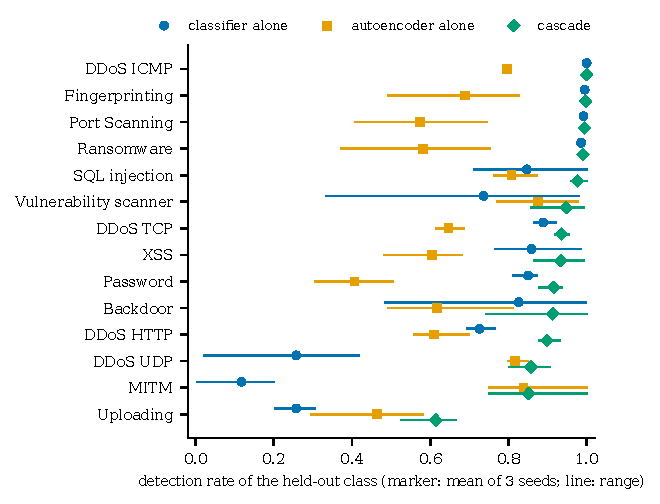
\includegraphics[width=\columnwidth]{figs/fig_zeroday.pdf}
\caption{Detection of each attack type when it is withheld from all training data, by stage. Classes are ordered by the cascade's mean detection rate.}
\label{fig:zeroday}
\end{figure}

\begin{table*}[t]
\centering
\caption{Leave-one-class-out detection, 10 clients, 0\% attackers, every row of the held-out class scored. Seeds 42 / 43 / 44.}
\label{tab:zeroday}
\small
\begin{adjustbox}{max width=\linewidth}
\begin{tabular}{lrlll}
\toprule
Held-out class & Rows & Classifier alone & Autoencoder alone & Cascade \\
\midrule
Backdoor & 24,167 & 0.486 / 0.996 / 0.997 & 0.493 / 0.550 / 0.810 & 0.743 / 0.998 / 0.998 \\
DDoS\_HTTP & 49,768 & 0.695 / 0.764 / 0.719 & 0.572 / 0.698 / 0.560 & 0.879 / 0.932 / 0.885 \\
DDoS\_ICMP & 68,758 & 1.000 / 1.000 / 0.999 & 0.786 / 0.802 / 0.800 & 1.000 / 1.000 / 1.000 \\
DDoS\_TCP & 50,062 & 0.865 / 0.921 / 0.879 & 0.640 / 0.686 / 0.615 & 0.933 / 0.953 / 0.921 \\
DDoS\_UDP & 121,567 & 0.416 / 0.021 / 0.334 & 0.849 / 0.799 / 0.799 & 0.905 / 0.803 / 0.866 \\
Fingerprinting & 872 & 0.995 / 0.994 / 0.994 & 0.826 / 0.747 / 0.492 & 0.998 / 0.998 / 0.997 \\
MITM & 406 & 0.148 / 0.200 / 0.005 & 0.764 / 1.000 / 0.751 & 0.803 / 1.000 / 0.751 \\
Password & 50,033 & 0.872 / 0.865 / 0.813 & 0.505 / 0.407 / 0.307 & 0.932 / 0.935 / 0.880 \\
Port\_Scanning & 20,213 & 0.998 / 0.988 / 0.989 & 0.570 / 0.745 / 0.409 & 0.999 / 0.993 / 0.992 \\
Ransomware & 9,885 & 0.984 / 0.990 / 0.982 & 0.621 / 0.753 / 0.374 & 0.990 / 0.994 / 0.988 \\
SQL\_injection & 50,981 & 0.828 / 0.713 / 0.999 & 0.764 / 0.871 / 0.787 & 0.961 / 0.970 / 0.999 \\
Uploading & 37,243 & 0.204 / 0.266 / 0.304 & 0.581 / 0.512 / 0.295 & 0.665 / 0.652 / 0.527 \\
Vuln.\ scanner & 50,044 & 0.980 / 0.894 / 0.335 & 0.880 / 0.976 / 0.772 & 0.992 / 0.993 / 0.859 \\
XSS & 15,172 & 0.823 / 0.986 / 0.767 & 0.680 / 0.650 / 0.483 & 0.943 / 0.991 / 0.867 \\
\midrule
Mean over 14 classes & & 0.735 / 0.757 / 0.723 & 0.681 / 0.728 / 0.590 & 0.910 / 0.944 / 0.895 \\
\bottomrule
\end{tabular}
\end{adjustbox}
\end{table*}
